\documentclass{hertieteaching}
%\usepackage{cancel}
%\usepackage{hyperref}
%
\title{Topic models}

\begin{document}

\maketitle

\begin{frame}{Plan}

\begin{itemize}
  \item Geometry
  \item Topic models, the very idea
  \item Latent Dirichlet Allocation
  \item Dirichlet distributions for beginners
  \item Training and output
  \item Interpretation
  \item Explaining topic prevalence
  \item The Structural Topic Model
\end{itemize}


\end{frame}

\begin{frame}{Word geometry}

Consider the $i$-th row of a document term matrix as a vector of proportions $P_i = [P_{i1} \ldots P_{iV}]$
\begin{itemize}
  \item (Make the proportions from counts $W_{iv}$ by dividing every count by the row sum)
\end{itemize}
This is the document's vocabulary profile

For fixed vocabulary, all possible documents live on a \textit{simplex}
\begin{itemize}
  \item The `corners' are where the document contains 100\% tokens of one vocabulary word
  \item There are $V$ of them, i.e. a lot\ldots
\end{itemize}
\end{frame}

\begin{frame}{Topic geometry}

Now consider the message $\theta_i = [\theta_{i1} \ldots \theta_{iK}]$ that we think the $i$-th document expresses.

This is a vector of $K$ \textit{topic proportions} for document $i$
\begin{itemize}
  \item From applying a dictionary
  \item From manual coding
  \item \ldots
\end{itemize}
This is the document's topic profile

For fixed vocabulary, all possible documents also live on a \textit{simplex}, but it
\begin{itemize}
  \item only has $K$ corners
  \item is embedded in the space of document profiles
\end{itemize}

Huge dimensionality reduction\ldots 

\end{frame}
\begin{frame}{Topic geometry}

\centerline{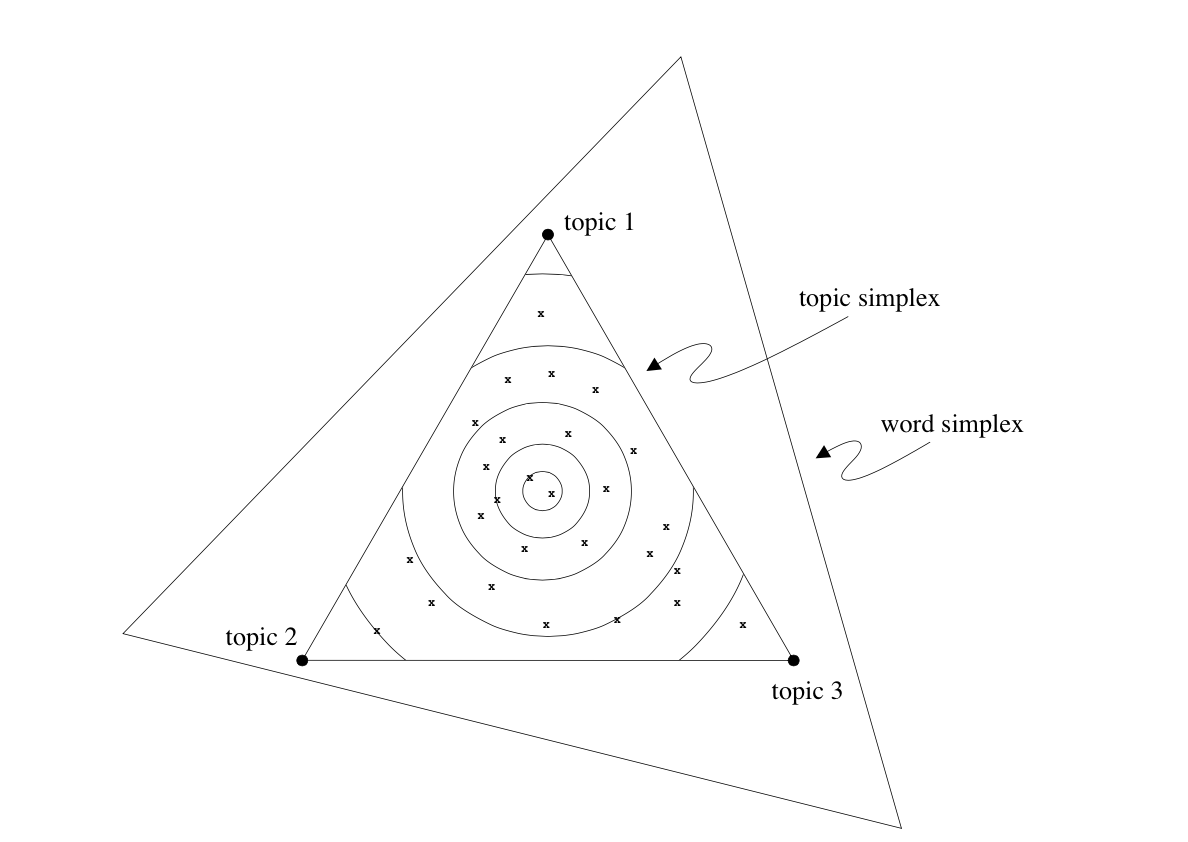
\includegraphics[scale=0.5]{pictures/topic-simplex}}
  
\end{frame}
\begin{frame}{Topic geometry}

The `corners' of the topic simplex represent the balance of words this topic generates 
\begin{itemize}
  \item i.e. a dictionary category
\end{itemize}
but with two differences to the ones we've been looking at. Each one 
\begin{itemize}
  \item contains an `entry' for every possible word, not just some of them
  \item expressed generatively, so we could `write' on that topic\\(by treating the entry as a set of multinomial parameters)
\end{itemize}

\end{frame}
\begin{frame}{Topic models}

Topic models answer the question: If we only knew $K$
\begin{itemize}
  \item What would a good set of topics be?
  \item What would be a good set of topic proportions be 
\end{itemize}
Basically 
\begin{itemize}
  \item $B = [\beta_1, \ldots, \beta_K]$~~ a matrix of word probabilities ($V$ words by $K$ topics)
  \item $\Theta = [\theta_1, \ldots, \theta_D]^T$~~ a matrix of topic proportions ($D$ documents by $K$ topics)
\end{itemize}

\bigskip
We'll look at the oldest and simplest way to answer these questions
\begin{itemize}
  \item Latent Dirichlet Allocation \parencite[a.k.a LDA,][]{Blei.etal2003}
\end{itemize}

\end{frame}

\begin{frame}{Dictionaries vs topic models}

\begin{columns}[T,onlytextwidth]
\column{0.5\textwidth}

\textsc{Dictionary-based content analysis}
\medskip

We know the dictionary

\bigskip
\begin{tikzpicture}
\node(W) at (1.5,0)  [var,label=below:$W$]{};
\node(Z) at (3,0)  [lat,label=below:$Z$]{};
\draw(Z) -- (W);
\draw[gray](1,-0.75) rectangle (3.75,0.5){};
\node[gray] at (4,-0.6){\small N};
\node(theta) at (4.5,0)  [lat,label=below:$\theta$]{};
\draw(theta) -- (Z);
\node(beta) at (-0.25, 0) [var,label=below:$\beta$]{};
\draw(beta) -- (W);
\draw(-0.75,-0.75) rectangle (0.5,0.5)[gray];
\node(labk) at (-0.95,-0.6)  []{{\color{gray}\small K}};
\end{tikzpicture}

\column{0.05\textwidth}
\column{0.45\textwidth}

\textsc{Topic model}
\medskip

We \textit{don't} know the dictionary

\bigskip
\begin{tikzpicture}
%\node(alpha) at (6,0) [var,label=right:$\alpha$]{};
%\draw(alpha) -- (theta);
%\node(eta) at (-2,0) [var,label=left:$\eta$]{}; 
%\draw(eta) -- (beta);
\node(W) at (1.5,0)  [var,label=below:$W$]{};
\node(Z) at (3,0)  [lat,label=below:$Z$]{};
\draw(Z) -- (W);
\draw[gray](1,-0.75) rectangle (3.75,0.5){};
\node[gray] at (4,-0.6){\small N};
\node(theta) at (4.5,0)  [lat,label=below:$\theta$]{};
\draw(theta) -- (Z);
\node(beta) at (-0.25, 0) [lat,label=below:$\beta$]{};
\draw(beta) -- (W);
\draw(-0.75,-0.75) rectangle (0.5,0.5)[gray];
\node(labk) at (-0.95,-0.6)  []{{\color{gray}\small K}};
\end{tikzpicture}

\end{columns}

\end{frame}
\begin{frame}{Latent Dirichlet Allocation}

We \textit{don't} know the dictionary, but 
we do have \textit{prior expectations}
\begin{itemize}
  \item about the $\beta$s
  \item about the $\theta$s
\end{itemize}

\bigskip
\begin{center}
\begin{tikzpicture}
\node(alpha) at (4.5,1.25) [var,label=right:$\alpha$]{};
\draw(alpha) -- (theta);
\node(eta) at (-0.25,1.25) [var,label=left:$\eta$]{}; 
\draw(eta) -- (beta);
\node(W) at (1.5,0)  [var,label=below:$W$]{};
\node(Z) at (3,0)  [lat,label=below:$Z$]{};
\draw(Z) -- (W);
\draw[gray](1,-0.75) rectangle (3.75,0.5){};
\node[gray] at (4,-0.6){\small N};
\node(theta) at (4.5,0)  [lat,label=below:$\theta$]{};
\draw(theta) -- (Z);
\node(beta) at (-0.25, 0) [lat,label=below:$\beta$]{};
\draw(beta) -- (W);
\draw(-0.75,-0.75) rectangle (0.5,0.5)[gray];
\node(labk) at (-0.95,-0.6)  []{{\color{gray}\small K}};
\draw[gray](0.75,-1) rectangle (5,0.75){};
%\node[gray] at (4,-0.6){\small N};
\end{tikzpicture}
\end{center}
\begin{align*}
  \beta_k & ~\sim~ \text{Dirichlet}(\eta)
  & \theta_d & ~\sim~ \text{Dirichlet}(\alpha)\\
  W_{i} & ~\sim~ \text{Multinomial}(\beta_{Z_i=k}, 1) & Z_i & ~\sim~ \text{Multinomial}(\theta_{d}, N)
\end{align*}

\end{frame}

\begin{frame}{Dirichlet distributions}

Two sources of information to figure out $\beta$
\begin{itemize}
  \item Prior: how `sparsely' populated is each topic with words?
  \item Likelihood: what words $W$ to we see?
\end{itemize}
Two sources of information to figure out $\theta$
\begin{itemize}
  \item Prior: how `sparsely' are documents populated with topics
  \item Likelihood: what topics $Z$ do we see?
\end{itemize}

We use a Dirichlet distribution for both priors:
\begin{itemize}
  \item Dirichlet distributions generate probabilities i.e. profiles on a simplex
\end{itemize}

\end{frame}
\begin{frame}{Dirichlet parameters}

% ggtern(data=as.data.frame(rdirichlet(1000, rep(1,3))),aes(V1,V2,V3)) + geom_point(alpha=0.2) + theme_minimal() + theme_hidelabels() + theme_hidetitles()+ theme_hidearrows(); ggsave("~/HertieSchool/courses/text-as-data/lectures/pictures/lda-alpha-1.pdf", width = 7.89/2, height = 7.64/2)

\begin{columns}[T,onlytextwidth]
\column{0.33\textwidth}
\begin{center}
$\alpha = [1, 1, 1]$

\bigskip
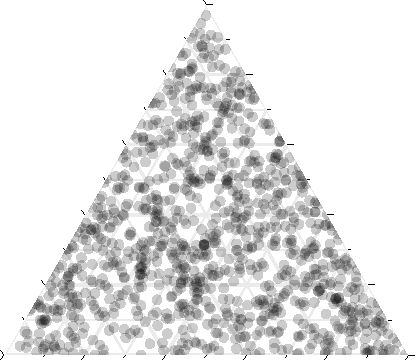
\includegraphics[scale=0.5]{pictures/lda-alpha-1-crop}
\end{center}

\column{0.33\textwidth}
\begin{center}
$\alpha = [10, 10, 10]$

\bigskip
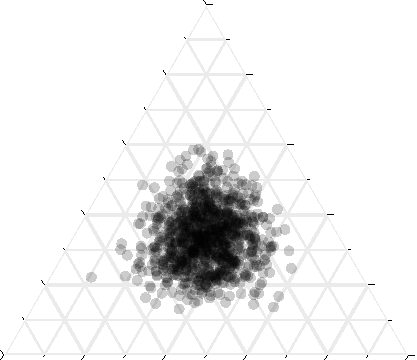
\includegraphics[scale=0.5]{pictures/lda-alpha-10-crop}
\end{center}

\column{0.33\textwidth}
\begin{center}
$\alpha = [0.1, 0.1, 0.1]$

\bigskip
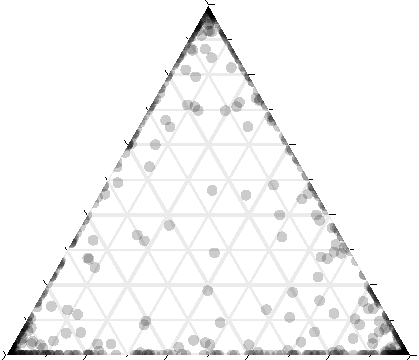
\includegraphics[scale=0.5]{pictures/lda-alpha-.1-crop}
\end{center}




\end{columns}


\end{frame}

\begin{frame}{Why Dirichlet?}

Because Multinomial! \pause Nice things about the Dirichlet distribution
\begin{itemize}
  \item It's \textit{conjugate} to the Multinomial
\end{itemize}
Let's (briefly) consider a special case: Beta (Dirichlet with 2 probabilities) and Binomial (Multinomial with 2 outcomes) 
\begin{itemize}
  \item \textit{two} possible topics (1 and 0) in proportions $[\theta_1, (1-\theta_1)]$  and a single document with $20$ words whose $Z$s are known: 15 $Z$=1s and 5 $Z$=0s
\end{itemize}
\begin{align*}
  P(\theta_1) & \propto \theta_1^{\alpha_1-1} (1-\theta_1)^{\alpha_2-1} & \text{Beta}\\
  P(Z_1 \ldots Z_{20} \mid \theta_1) & \propto \prod^{20}_i \theta_1^{Z_i} (1-\theta_1)^{Z_i}\\
   & \propto \theta_1^{15} (1-\theta_1)^{5} & \text{Binomial}\\
 P(\theta_1 \mid Z_1 \ldots Z_{20}) & \propto \theta_1^{(15 + \alpha_1 - 1)} (1-\theta_1)^{(5 + \alpha_2 - 1)} & \text{Beta again!}
\end{align*}

\end{frame}

\begin{frame}{Why Dirichlet?}

% fnt <- "Minion Pro Caption"
%minpro <- theme(axis.text.x = element_text(family=fnt),
%      axis.title.x = element_text(family=fnt),
%      axis.text.y = element_text(family=fnt),
%      axis.title.y = element_text(family=fnt),
%      plot.title = element_text(family=paste(fnt)),
%      legend.text=element_text(family=fnt),
%      legend.title=element_text(family=fnt))

% vv <- data.frame(x = seq(0,1,by=0.01), `prior(10)` = dbeta(seq(0,1,by=0.01), 10, 10), `prior(.1)` = dbeta(seq(0,1,by=0.01), .1, .1), `posterior(.1)` = dbeta(seq(0,1,by=0.01), 15+.1-1, 5+.1-1), `prior(1)` = dbeta(seq(0,1,by=0.01), 1, 1), `posterior(10)` = dbeta(seq(0,1,by=0.01), 15+10-1, 5+10-1), `posterior(1)` = dbeta(seq(0,1,by=0.01), 15+1-1, 5+1-1))

% pivot_longer(vv, -x, names_to = "Distribution", values_to = "P") %>% ggplot(aes(x, P, color = Distribution, linetype = Distribution)) + geom_line() + geom_vline(xintercept = 3/4, linetype = "dotted") + theme_minimal() + labs(y = "Density", x = "Theta 1") + scale_linetype_manual(values = rep(c("dashed", "solid"), each = 3), guide = FALSE) + scale_color_manual(values = c("brown3", "chartreuse3", "blue3", "brown3", "chartreuse3", "blue3"), labels = c("Posterior (alpha=0.1)", "Posterior (alpha=1)", "Posterior (alpha=10)", "alpha=0.1", "alpha=1", "alpha=10")) + minpro 
% ggsave("~/HertieSchool/courses/text-as-data/lectures/pictures/beta_binomial-3.pdf", width = 7, height = 2.5, device = cairo_pdf)

\bigskip

\centerline{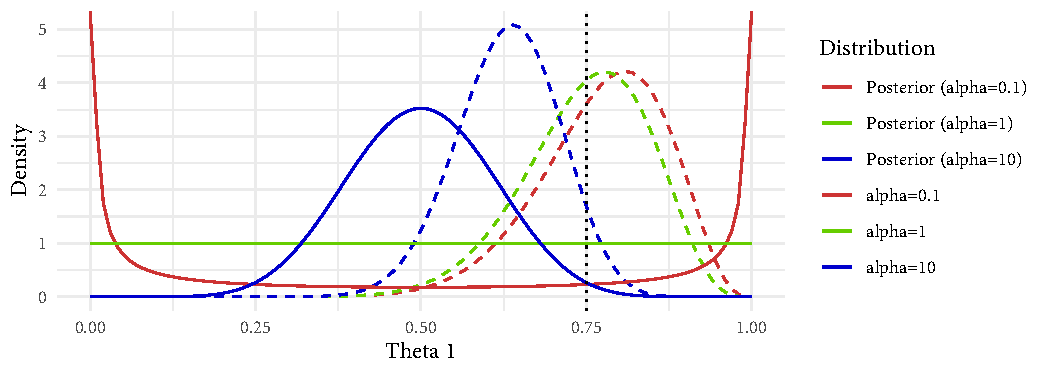
\includegraphics[scale=0.8]{pictures/beta_binomial-3}} 
 
Prior distributions are solid lines and the resulting posterior distributions over $\theta$ for 15 $Z$=1 and 5 $Z$=0 are dashed.
 
\end{frame}


\begin{frame}{Topic model training}

Topic models can be quite time consuming to estimate. 
\begin{itemize}
  \item Lots of coupled unknowns all at once
\end{itemize}

Intuition:
\begin{itemize}
  \item Any set of parameters make the observed word counts more or less probable
  \item If we knew the $Z$'s then estimating $\beta$ and $\theta$ would be straightforward
  \item If we new $\beta$ and $\theta$ then estimating $Z$ would be straightforward
  \item So alternate between these steps
\end{itemize}
This simple approach is called \textit{Gibbs sampling}

A more complete machine learning course will tell you all about; we won't linger\ldots 

\end{frame}

\begin{frame}{Topic models: $\beta$}

\medskip
\centerline{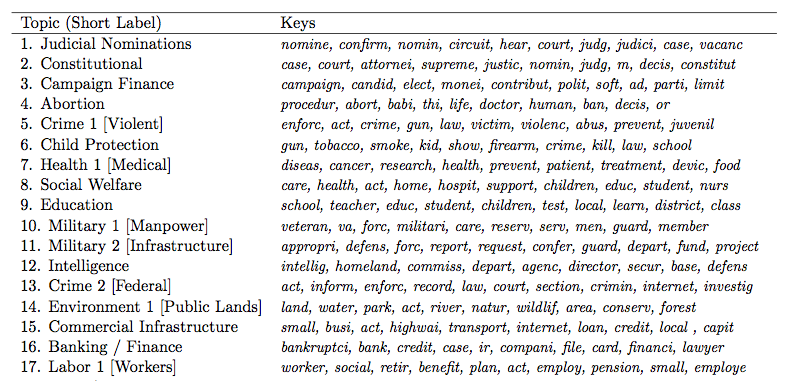
\includegraphics[scale=0.4]{pictures/topic-words}}
From \textcite{Quinn.etal2007}\\
Note: only the top most probable words are shown and topic labels are manually assigned.

\end{frame}

\begin{frame}{Topic models: $\theta_k$}

\centerline{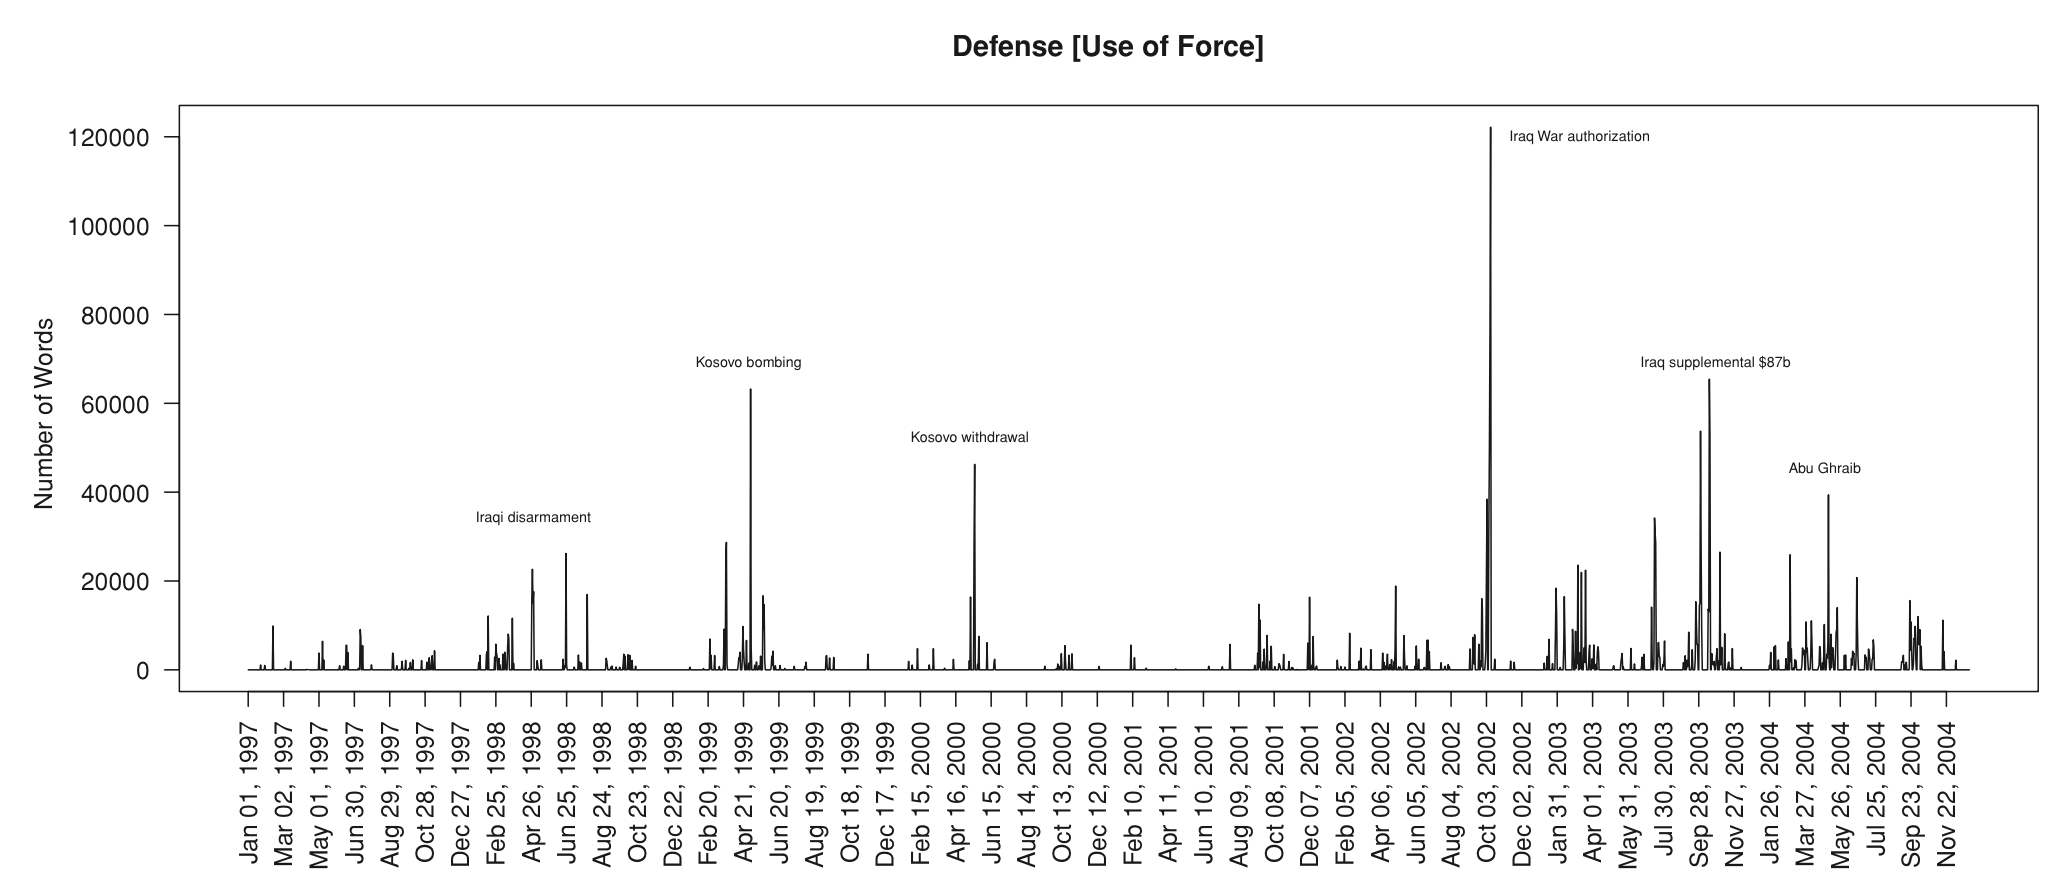
\includegraphics[scale=0.35]{pictures/defence-topic-quinn}}

From \textcite{Quinn.etal2007}

\end{frame}


\begin{frame}{Interpreting topics}

Ideally we'd like to be able to say: ``make this one about defense''

Unfortunately, that level of high level control is an unsolved problem

We can only \textit{after the fact} assign our own labels the topics, and hope some are topics that we want.

\bigskip
Are they good, these topics?
\begin{itemize}
  \item often better the \textit{statistical} properties of the model the less interpretable it tends to be \parencite{Chang.etal2009}
  \item Clearly we're missing something with the model structure\ldots
\end{itemize}

\end{frame}

\begin{frame}{Explaining topic prevalence}

\begin{columns}[T,onlytextwidth]
\column{0.5\textwidth}
Often we want to both \textit{measure} but also \textit{explain} the prevalence of topic mentions

\medskip
Example: What are the effects of a Japanese house electoral reform on candidate platforms? \parencite{Catalinac2018}

\medskip
\begin{itemize}
  \item Fit a topic model to LDP platforms
  \item Extract two topics that look like `pork' and `policy'
  \item Average these per year and plot
  \item Compare relative prevalence to electoral change timeline
\end{itemize}

\column{0.05\textwidth}
\column{0.45\textwidth}
\centerline{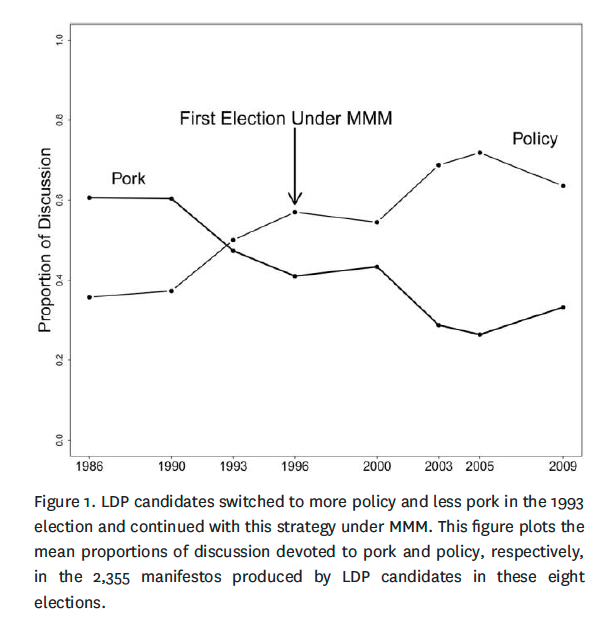
\includegraphics[scale=0.27]{pictures/jpcontent}}
\end{columns}





        
\end{frame}


\begin{frame}{Structural topic model}

If we like some of the topics, we might want to know how they vary with external information, e.g.
\begin{itemize}
  \item How does rate of topic 3, say `defence', change with the party of the speaker?
\end{itemize} \pause
This is a regression model \parencite{Roberts.etal2014} with
\begin{itemize}
  \item speaker party indicator, convariates etc. as $X$ (observed)
  \item proportion of the speech assigned to topic 3 as $\theta_3$ (inferred, not observed)
  \item The words $W$ (observed)
\end{itemize}

\begin{center}
\begin{tikzpicture}
\node(alpha) at (4.5,1.25) [var,label=right:$\phi$]{};
\draw(alpha) -- (theta);
\node(eta) at (-0.25,1.25) [var,label=left:$\eta$]{}; 
\draw(eta) -- (beta);
\node(W) at (1.5,0)  [var,label=below:$W$]{};
\node(Z) at (3,0)  [lat,label=below:$Z$]{};
\draw(Z) -- (W);
\draw[gray](1,-0.75) rectangle (3.75,0.5){};
\node[gray] at (4,-0.6){\small N};
\node(theta) at (4.5,0)  [lat,label=below:$\theta$]{};
\draw(theta) -- (Z);
\node(beta) at (-0.25, 0) [lat,label=below:$\beta$]{};
\draw(beta) -- (W);
\draw(-0.75,-0.75) rectangle (0.5,0.5)[gray];
\node(labk) at (-0.95,-0.6)  []{{\color{gray}\small K}};
\draw[gray](0.75,-1) rectangle (6.5,0.75){};
\node(X) at (6,0) [var,label=below:$X$]{};
\draw(X) -- (theta);
%\node[gray] at (4,-0.6){\small N};
\end{tikzpicture}
\end{center}

\end{frame}


\begin{frame}{Structural topic model}

Having a topic model allows us to get contrast vocabulary \textit{within topic} too. 

Here's contrasting usage when talking about Guatanamo Bay in a Bush era data set

\centerline{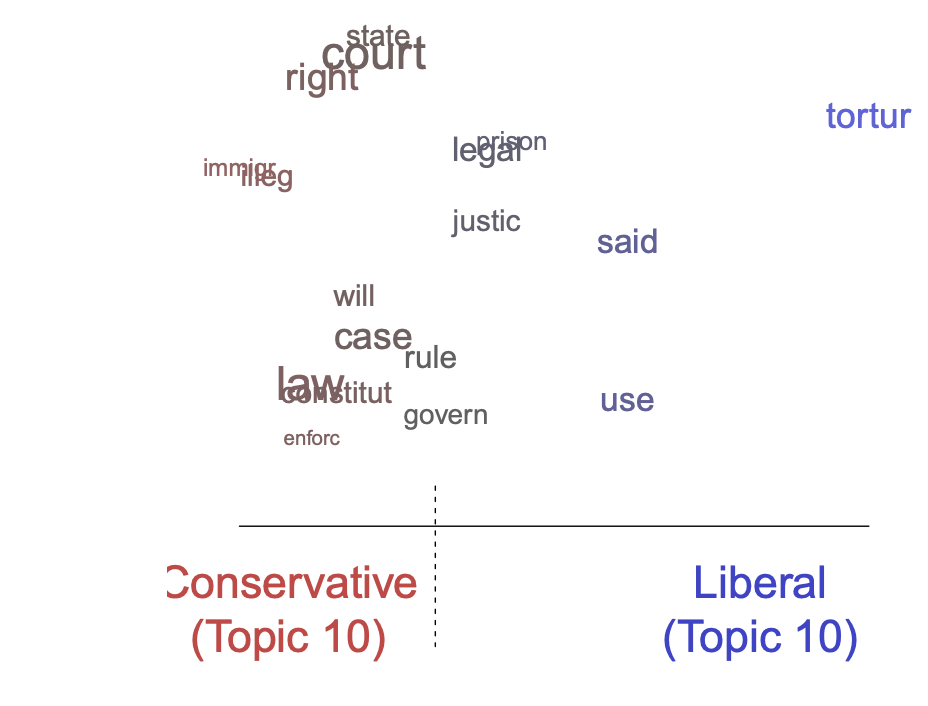
\includegraphics[scale=0.45]{pictures/comparisons-stm}}
        
\end{frame}
\begin{frame}{Even more topic models}

There's a small industry developing new types of topic model
\begin{itemize}
  \item A brief search will acquaint you with more than enough to play with
\end{itemize}
Check if they have stable code!

\bigskip
We'll look closer into topic model evaluation and related matters next week!
	
\end{frame}




%## Topic Models
%
%We'll start with a Latent Dirichlet Allocation topic model and then
%consider some useful extensions.
%
%LDA estimates
%
%- A complete distribution of words for each topic ($\beta$)
%- Estimated proportions of tokens in each document in each topic
%  ($\theta$)
%
%and requires from us
%
%- A document term matrix (always)
%- Hyperparameter values for topic proportions and word generation
%  probabilities (sometimes)
%
%Stacks and stacks of parameters...
%
%## Latent Dirichlet Allocation
%
%```{r, out.width='80%', fig.cap = "Blei (slides)"}
%knitr::include_graphics("pictures/topic-model.png")
%```
%
%
%
%## Parameters and hyperparameters
%
%- W and Z are multinomial distributions
%- $\theta$ and $\beta$ are Dirichlet distributions
%- $\alpha$ and $\eta$ are 'hyperparameters' for Dirichlet parameters
%
%Dirichlet distributions generate probability distributions over fixed
%numbers of categories
%
%*Their* parameters control the shape and sparsity of what is generated.
%
%## Latent Dirichlet Allocation Components
%Given dimensions:
%
%- N documents, K different topics, V unique words
%
%We want the following matrices:
%
%- $W = N \times V$ document-term matrix (observed)
%- $\theta = N \times V$ matrix with row $\theta_i = (\theta_{i1},\ldots,\theta_{iV})$
%  
%  - $\theta_{iv}$: Proportion of document $i$ allocated to topic k
%
%- $\beta = V \times K$ matrix with row $\beta_v = (\beta_{v1}, \ldots, \beta_{vK})$
%  - $\beta_{vk}$: Probability of using word v, if topic k is chosen
%  
%- $\alpha$ = K length population prior for $\theta$
%
%Objective function: f(X, $\beta, \theta, \alpha)$
%
%
%## LDA Generative Model
%
%When writing a word ($m$) for document $i$:
%$$
%\begin{aligned}
%P(\theta_i | \alpha) &= \text{Dirichlet}(\alpha) && \text{(Pick potential topics $\theta_i$)}\\
%P(Z_{im} | \theta_i)  &= \text{Multinomial}(1, \theta_i) && \text{ (Pick a topic to mention)}\\
%W_{im} | \beta_v, Z_{im} &= \text{Multinomial}(1, \beta_v)  && \text{ (Pick a word from topic $z_{im}$) }\\
%P(\beta_v) &= \text{Dirichlet}(\eta)  && \text{(Prior on topics)}\\
%P(\alpha_v) &= \text{Gamma}(\alpha,\beta)  && \text{(Prior on document proportions)}
%\end{aligned}
%$$
%
%with
%
%P($\beta$, $\theta$, Z, $\alpha$ | W) $\propto$  P($\beta$ | $\eta$) $\cdot$ P($\theta$|$\alpha$) $\cdot$ P(Z | $\theta$) $\cdot$ P(W | $\beta$, Z)
%
%
%## Intuition on LDA
%
%P($\beta$, $\theta$, Z, $\alpha$ | W) $\propto$  P($\beta$ | $\eta$) $\cdot$ P($\theta$|$\alpha$) $\cdot$ P(W | $\theta$) $\cdot$ P(W | $\beta$, Z)
%
%Remember rows of $\beta$ and $\theta$ must sum to 1!
%
%P(W | $\beta$, Z) Favors co-occurring words, segregated topics
%
%- $\beta$ = (0.5,0.5,0,0) vs $\beta$ = (0.25,0.25,0.25,0.25)
%
%P(Z | $\theta$): Higher if $\theta$ is concentrated,i.e. fewer potential topics
%
%- $\theta$ = (0.5,0.5, 0, 0) vs. $\theta$ = (0.25, 0.25, 0.25, 0.25)
%
%Joint distribution favors sparse topics, small topic clusters
%
%But data often need a larger number of topics to assign small topic clusters to data
%
%Priors on $\alpha$ and $\eta$ regulate these tendencies
%
%## $\alpha = 10$
%```{r, out.width='90%'}
%knitr::include_graphics("pictures/dirichlet-alpha10.png")
%```
%
%## $\alpha = 0.1$
%```{r, out.width = '90%'}
%knitr::include_graphics("pictures/dirichlet-alpha-tenth.png")
%```
%
%Happily these are often estimated for us, or modeled with covariates (in the Structural Topic Model).
%
%
%<!-- %SNTV-MMD: Single nontransferable vote, multimember district -->
%<!-- %More competition within party, as majority-seeking parties run multiple candidates in each district -->
%<!-- % MMM: Mixed member district: PR + single member districts -->
%
%## What are these topics anyway?
%
%Construct validity: What are the most probable 
%words to be generated in each topic?
%
%```{r, fig.cap = "(Quinn et al., 2007)", out.width='80%'}
%knitr::include_graphics("pictures/topic-words.png")
%```
%
%## What are these topics anyway?
%
%We can also ask for the most *distinctive*
%
%Randomly select documents from each topic with a high proportion
%of that topic, then read and manually assign a label
%
%## What are these topics anyway?
%
%Validate with external events (predictive validity)
%
%```{r, fig.cap = "(Quinn et al., 2007)", out.width='100%'}
%knitr::include_graphics("pictures/grimmerimmig.pdf")
%```
%
%## What are these topics anyway?
%
%Construct validity: How do these topic relate to each other?
%
%```{r, out.width='70%'}
%knitr::include_graphics("pictures/topic-clustering.png")
%```
%
%## Number of topics?
%
%> The results presented in this paper ... assume there are 43 
%> topics present in the data. I varied the number of assumed topics
%> from only five topics, up to 85 different topics. Assuming too few
%> topics resulted in distinct issues being lumped together, whereas 
%> too many topics results in several clusters referring to the same
%> issues. During my tests, 43 issues represented a decent middle
%> ground. 
%> (Grimmer 2010, p.12)
%
%## Number of topics?
%
%A typical result
%
%```{r, out.width='80%'}
%knitr::include_graphics("pictures/heldout-lda.png")
%```
%
%## The interpretability dilemma
%
%There are two natural metrics for evaluating topic models (or any other kind of computer assisted text analysis
%
%- Statistical performance, e.g. held-out likelihood
%- Substantive usefulness, e.g. topic coherence
%
%Experiments by @Chang.etal2009 using
%
%- word intrusion (which word does not belong?)
%- topic intrusion (which topic does not belong?)
%
%suggest that these are *negatively* correlated.
%
%## The interpretability dilemma
%
%```{r, out.width = "95%", fig.cap = "(Chang 2009)"}
%knitr::include_graphics("pictures/chang2009.png")
%```
%
%## Gamson and Modigliani revisited
%
%```{r, out.width = '100%', fig.cap = "Jacobi et al (2014)"}
%knitr::include_graphics("pictures/nested-topics-nuclear.png")
%```
%
%## Explaining topic prevalence: A case study
%
%Catalinac (2016) Examines the effect of electoral reform
%
%- Before 1994: SNTV-MMD (more intraparty competition)
%- After 1994: Mixed member majoritarian (PR + SMD)
%
%LDA on N = 7497 candidate manifestos for Diet 1950-2009
%
%- Hand transcribed, OCR failed
%- Things are complicated in Japanese!
%
%Characterizing campaigns across 50+ years
%
%- What do candidates talk about?
%- How did electoral reform change incentives?
%- Why increasing interest in military foreign action?
%
%## Japanese Manifestos
%
%```{r, out.width = '95%'}
%knitr::include_graphics("pictures/jpmanifesto.png")
%```
%
%## Japanese Manifesto Topics
%
%```{r, out.width = '110%'}
%knitr::include_graphics("pictures/jptopic.png")
%```
%
%## Manifesto Content over Time
%
%```{r, out.width = '70%'}
%knitr::include_graphics("pictures/jpcontent.png")
%```
%
%## Foreign Policy Content
%
%```{r, out.width = '60%'}
%knitr::include_graphics("pictures/jpforeign.png")
%```
%
%## Doing it all at once
%
%Structural topic model [@Roberts.etal2014].
%
%```{r, out.width = '80%'}
%knitr::include_graphics("pictures/lda-stm2.pdf")
%```
%
%## Doing it all at once
%
%```{r, out.width = '90%', fig.cap = "(Nielsen 2013)"}
%knitr::include_graphics("pictures/nielsen-stm.png")
%```
%
%## Doing it all at once
%
%```{r, out.width = '90%', fig.cap = "(Nielsen 2013)"}
%knitr::include_graphics("pictures/nielsen-two-props.png")
%```
%
%## Practical issues: Baerg and Lowe
%
%A timeline:
%
%- Paper and basic results sent to ACL workshop (wins prize)
%- Inflated to poli-sci length paper and sent to review
%- Reviewers do not believe topics measure what we say they measure
%- We validate manually, and compare to other measures
%- Reviewers do not believe topics measure what we say they measure
%- We validate manually, and compare to other measures
%- (repeat)
%
%Publish.
%
%Disagreements were *all* about measurement
%
%##
%
%```{r, out.width = '90%'}
%knitr::include_graphics("pictures/filedrawer.jpg")
%```
%




\begin{frame}[allowframebreaks]
\frametitle{References}
\printbibliography	
\end{frame}

\end{document}